\begin{python}
    self.dashboard <= w.label('Checkbox', typo='headline4', style=flex_title)
    self.dashboard <= w.checkbox(
        'Checkbox',
        options=[[f'chb-{i}', False] for i in range(4)],
        on_change=self.on_checkbox,
        id='my_checkbox',
    )
    self.dashboard <= w.label(
        f'', id='for_checkbox', typo=f'body1', style=flex
    )


def on_checkbox(self):
    value = w.get_value('my_checkbox')
    document.select_one('#for_checkbox').html = f'Checkbox Changed: {value}'
\end{python}


\begin{figure}[H]
\begin{centering}
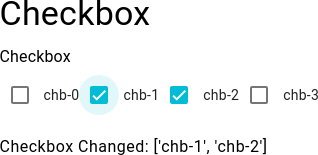
\includegraphics[scale=0.5]{Cap4/Figures/widgets/checkbox.png}
\par\end{centering}
\caption[Brython Radiant: Checkbox]{Brython Radiant: Checkbox.}
\label{fig:radiant_checkbox}
\end{figure}